\section{Tasks Status} % Seções são adicionadas para organizar sua apresentação em blocos discretos, todas as seções e subseções são automaticamente exibidas no índice como uma visão geral da apresentação, mas NÃO são exibidas como slides separados.

%----------------------------------------------------------------------------------------


\begin{frame}
  \frametitle{General Tasks Status}

  \centering
  \renewcommand{\arraystretch}{1.15}

  \begin{table}
    \begin{tabular}{|p{0.58\textwidth}|c|p{0.22\textwidth}|}
      \hline
      \textbf{Task} & \textbf{Status} &  \\
      \hline

      \hspace{1.2em}\textbf{2026-06 RETINHA presentation}
      & \inprogressqqq & \href{https://www.overleaf.com/project/69fcf33ccbe729b0fca5157b}{Link} \\
      \hline

      \hspace{1.2em}\textbf{2026-06 Scientific report}
      & \inprogressqq  & \href{https://www.overleaf.com/project/69fcf33ccbe729b0fca5157b}{Link} \\
      \hline

      \hspace{1.2em}\textbf{2026-11 Journal Article}
      & \pending & \href{https://www.overleaf.com/project/69fce32953269e6b2073b03c}{Link} \\
      \hline

      \hspace{1.2em}\textbf{Dissertation}
      & \inprogressq & \href{https://www.overleaf.com/project/69fcf3a033b4cc5dcfcf23ff}{Link} \\
      \hline

    \end{tabular}
  \end{table}


  \begin{table}
    \begin{tabular}{|p{0.58\textwidth}|c|p{0.22\textwidth}|}
      \hline
      \textbf{Task} & \textbf{Status} &  \\
      \hline

      \hspace{1.2em}\textbf{Journal Club - Automations}
      & \inprogressqqqq & \\
      \hline

    \end{tabular}
  \end{table}
\end{frame}


\begin{frame}
  \frametitle{Tasks Status}

  % Ajustes úteis em tabelas no Beamer
  \centering
  \renewcommand{\arraystretch}{1.15} % mais espaço vertical entre linhas

  \begin{table}

\begin{tabular}{|p{0.58\textwidth}|c|p{0.22\textwidth}|}
\hline
\textbf{Task} & \textbf{Status} & \textbf{Link} \\
\hline
\textbf{Walkthrough Atlas experiment ins1759506} & & \\
\cline{1-2}
\hspace{1.2em}\small$\hookrightarrow$ Centrality Bins (pt integrated) & \done & \href{https://high-energy-physics-research.github.io/experimental-correlation-uncertainty/studies.html?nb=10.17182\%2FHEPData-ins1759506-v1-csv\%2Fanalysis\%2F01_Centrality_Bins-PB-PB_comp_pp.ipynb}{Notebook} \\
\cline{1-2}
\hspace{1.2em}\small$\hookrightarrow$ Pt Bins & \done & \href{https://high-energy-physics-research.github.io/experimental-correlation-uncertainty/studies.html?nb=10.17182\%2FHEPData-ins1759506-v1-csv\%2Fanalysis\%2F02_Pt_Bins-PB-PB_comp_pp.ipynb}{Notebook} \\
\cline{1-2}
\hspace{1.2em}\small$\hookrightarrow$ RAA & \done & \href{https://high-energy-physics-research.github.io/experimental-correlation-uncertainty/studies.html?nb=10.17182\%2FHEPData-ins1759506-v1-csv\%2Fanalysis\%2F03_RAA_Analysis.ipynb}{Notebook} \\
\cline{1-2}
\hspace{1.2em}\small$\hookrightarrow$ Understand the origin of the sistematic correlated information & \pending & \\
\cline{1-2}
\textbf{Walkthrough Thiago's work} & & \\
\cline{1-2}
\hspace{1.2em}\small$\hookrightarrow$ Scaled Spectra & \inprogressqqqqq & \\
\cline{1-2}
\hline
\end{tabular}
\end{table}

\end{frame}


\begin{frame}
  \frametitle{Correlated Uncertainty Study Tasks Status}

  \centering
  \renewcommand{\arraystretch}{1.15}
  \begin{table}

\begin{tabular}{|p{0.58\textwidth}|c|p{0.22\textwidth}|}
\hline
\textbf{Task} & \textbf{Status} & \textbf{Link} \\
\hline
\textbf{Scaled Spectra With Correlated Uncertainty} & & \\
\cline{1-2}
\hspace{1.2em}\small$\hookrightarrow$ Implement effects from correlated uncertainty in scaled spectra & \inprogressqqqq & \href{https://high-energy-physics-research.github.io/Gaussian-Process-Research/studies.html?nb=Estudo\%2FFase+01+-+Prova+de+Conceito\%2FModel-to-data-Comparison.ipynb}
     {Notebook}\\
\cline{1-2}
\hspace{1.2em}\small$\hookrightarrow$ Analyse effects from correlated uncertainty in scaled spectra & \inprogressqqq & \\
\cline{1-2}
\hline
\end{tabular}
\end{table}
\end{frame}


\begin{frame}
  \frametitle{Correlated Uncertainty Study Tasks Status}

  \centering
  \renewcommand{\arraystretch}{1.15}
  \begin{table}

\begin{tabular}{|p{0.58\textwidth}|c|p{0.22\textwidth}|}
\hline
\textbf{Task} & \textbf{Status} & \textbf{Link} \\
\hline
\textbf{Correlated uncertainty study} & & \\
\cline{1-2}
\hspace{1.2em}\small$\hookrightarrow$ Model GP uncertainty prediction and compare with Atlas experiment ins1759506 & \inprogressqq & \href{https://high-energy-physics-research.github.io/Gaussian-Process-Research/studies.html?nb=Estudo\%2FFase+01+-+Prova+de+Conceito\%2FModel-to-data-Comparison.ipynb}
     {Notebook}\\
\cline{1-2}
\hspace{1.2em}\small$\hookrightarrow$ Check effect on Pt Scaled Spectra (Thiago's work) & \inprogressqqqq & \\
\cline{1-2}
\hline
\end{tabular}
\end{table}
\end{frame}

% \begin{frame}
%   \frametitle{Tasks Status}

%   % Ajustes úteis em tabelas no Beamer
%   \centering
%   \renewcommand{\arraystretch}{1.15} % mais espaço vertical entre linhas

%   \begin{table}

% \begin{tabular}{|p{0.58\textwidth}|c|p{0.22\textwidth}|}
% \hline
% \textbf{Task} & \textbf{Status} & \textbf{Link} \\
% \hline

% \textbf{Model correlated uncertainty in Scaled Spectra} & &
% \multirow{4}{*}{\centering \href{https://high-energy-physics-research.github.io/Gaussian-Process-Research/studies.html?nb=Estudo\%2FFase+01+-+Prova+de+Conceito\%2FModel-to-data-Comparison.ipynb}
%      {Notebook}} \\
% \cline{1-2}
% \hspace{1.2em}\small$\hookrightarrow$ Walkthrough Atlas experiment ins1759506 & \done & \\ 
% \cline{1-2}
% \hspace{1.2em}\small$\hookrightarrow$ Check uncertainty prediction in Atlas experiment ins1759506 & \inprogress & \\
% \cline{1-2}
% \hspace{1.2em}\small$\hookrightarrow$ Check effect on pt scaled spectra (Thiago's work) & \inprogress & \\
% \cline{1-2}
% \hline
% \end{tabular}
% \end{table}
% \end{frame}

%----------------------------------------------------------------------------------------


% \begin{frame}
%   \frametitle{Tasks Status}

%   \centering
%   \renewcommand{\arraystretch}{1.15}

%   \begin{table}
%     \begin{tabular}{|p{0.58\textwidth}|c|p{0.22\textwidth}|}
%       \hline
%       \textbf{Task} & \textbf{Status} &  \\
%       \hline

%       \textbf{Analisar toy model} &  &  \\
%       \hline

%       \hspace{1.2em}\small$\hookrightarrow$ 
%       & \done &  \\
%       \hline

%       \hspace{1.2em}\small$\hookrightarrow$ 
%       & \done &  \\
%       \hline

%       \hspace{1.2em}\small$\hookrightarrow$ 
%       & \done &  \\
%       \hline

%       \hspace{1.2em}\small$\hookrightarrow$ 
%       & \done &  \\
%       \hline

%       \hspace{1.2em}\small$\hookrightarrow$ 
%       & \inprogress &  \\
%       \hline

%       \hspace{1.2em}\small$\hookrightarrow$ 
%       & \pending &  \\
%       \hline

%     \end{tabular}
%   \end{table}
% \end{frame}

% \begin{frame}
%   \frametitle{Tasks Status}

  % Ajustes úteis em tabelas no Beamer
%   \centering
%   \renewcommand{\arraystretch}{1.15} % mais espaço vertical entre linhas

%   \begin{table}

% \begin{tabular}{|p{0.58\textwidth}|c|p{0.22\textwidth}|}
% \hline
% \textbf{Task} & \textbf{Status} & \textbf{Link} \\
% \hline

% \textbf{Escrever projeto} & &
% \multirow{4}{*}{\centering \href{https://www.overleaf.com/project/696e133a1101ac682ea3dd98}{Projeto}} \\
% \cline{1-2}

% \hspace{1.2em}\small$\hookrightarrow$ Definir escopo e objetivos & \done & \\
% \cline{1-2}

% \hspace{1.2em}\small$\hookrightarrow$ Esboçar introdução (motivação + observáveis) & \done & \\
% \cline{1-2}

% \hspace{1.2em}\small$\hookrightarrow$ Cronograma & \done & \\
% \cline{1-2}

% \hspace{1.2em}\small$\hookrightarrow$ Selecionar bibliografia & \done & \\
% \cline{1-2}

% \hspace{1.2em}\small$\hookrightarrow$ Listar método: GP  & \done & \\
% \cline{1-2}

% \hspace{1.2em}\small$\hookrightarrow$ Listar método: Bayesian Inferente  & \done & \\
% \cline{1-2}

% \hspace{1.2em}\small$\hookrightarrow$ Listar objetivos & \done & \\

% \hline
% \end{tabular}
% \end{table}
% \end{frame}

% \begin{frame}{Uma imagem}
%     \frametitle{Historical Records}
%     In addition, it is possible to retrieve the full search history by running the script directly via GitHub Actions.
%    \begin{figure}[h]
%        \centering
%        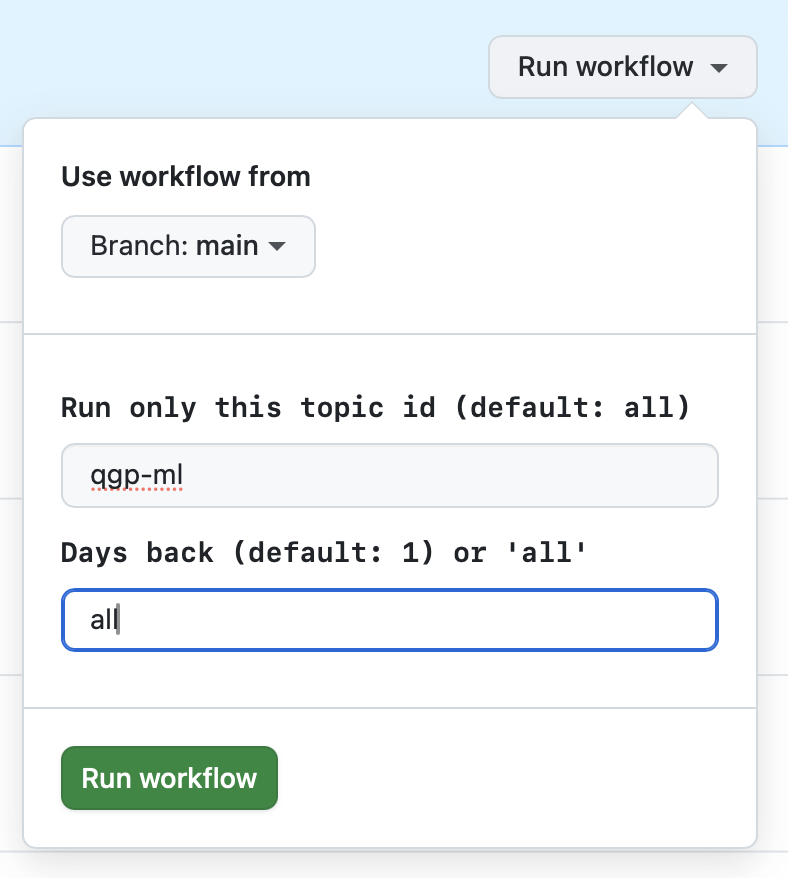
\includegraphics[width=0.3\textwidth]{img/github_topic_history.png}
%        \caption{GitHub Actions interface illustrating how the workflow can be executed to retrieve the full search history for a specific topic.}
%        \label{fig:github_topic_history}
%    \end{figure}
% \end{frame}
%----------------------------------------------------------------------------------------

% \begin{frame}
% 	\frametitle{Texto em tópicos}
%      Lorem ipsum dolor sit amet, consectetur adipiscing elit:
%     \begin{itemize}
%         \item Lorem ipsum dolor sit amet.
%         \item Lorem ipsum dolor sit amet.
%     \end{itemize}
	
% \end{frame}


